\documentclass[10pt, article, natbib]{IEEEtran}
\IEEEoverridecommandlockouts
\usepackage[utf8]{inputenc}
\usepackage[spanish]{babel}
\usepackage[T1]{fontenc}
\usepackage{amsmath}
\usepackage{fancyhdr}
\usepackage{mathtools}
\usepackage{tikz}
\usepackage{pgfplots}
\pgfplotsset{compat=1.8}

\usepackage{courier} %% Sets font for listing as Courier.
\usepackage{listings, xcolor}
\lstset{
tabsize = 4, %% set tab space width
showstringspaces = false, %% prevent space marking in strings, string is defined as the text that is generally printed directly to the console
numbers = left, %% display line numbers on the left
commentstyle = \color{green}, %% set comment color
keywordstyle = \color{blue}, %% set keyword color
stringstyle = \color{red}, %% set string color
rulecolor = \color{black}, %% set frame color to avoid being affected by text color
basicstyle = \small \ttfamily , %% set listing font and size
breaklines = true, %% enable line breaking
numberstyle = \tiny,
}

\pagestyle{fancy}
\fancyhf{Universidad Nacional de Costa Rica}
\rhead{\thepage}
\lhead{Linux vs Windows Escritura}
\rfoot{EIF-212 Sistemas Operativos}
\lfoot{I-2023}

\def\changemargin#1#2{\list{}{\rightmargin#2\leftmargin#1}\item[]}
\let\endchangemargin=\endlist

\DeclarePairedDelimiter\ceil{\lceil}{\rceil}
\DeclarePairedDelimiter\floor{\lfloor}{\rfloor}
\makeatletter
\renewcommand*\l@section{\@dottedtocline{1}{1.5em}{2.3em}}
\makeatother

\title{Tarea Linux vs Windows Escritura}
\author{Diego Quirós Artiñano}

\onecolumn
\begin{document}
\maketitle
\thispagestyle{fancy}

Esta tarea se basa en escribir un millón de 'a'. Cada vez que se escribe se tiene que abrir el documento, escribir y volver a cerrar el documento. Para esto se implementó el siguiente código en Java.

\begin{lstlisting}[language = Java , frame = trBL , firstnumber = last , escapeinside={(*@}{@*)}]
import java.io.File;
import java.io.FileWriter;
import java.io.IOException;

public class a
{
    public static void main(String[] args)
    {   
    		File file = new File("a.txt");
    		try {
    			file.createNewFile();
    		} catch (IOException e) {
    			System.out.println("An error has ocurred.");
    			e.printStackTrace();
    		}
    		for (int i = 0; i < 1000000; i++) {
    			try {
				FileWriter file_writer = new FileWriter(file, true);
				file_writer.write("a");
				file_writer.close();    			
    			} catch (IOException e) {
				System.out.println("An error has ocurred.");
				e.printStackTrace();    			
    			}
    		}
    }
}
\end{lstlisting}

\begin{tikzpicture}
\begin{axis}[title = Tiempo de ejecución Linux vs. Windows,
xbar, xmin=0,
width=0.8\textwidth, height=0.6\textwidth,
xlabel={Time (s)},
symbolic y coords={%
    Promedio,
    {Tercera Prueba},
    {Segunda Prueba},
    {Primera Prueba}},
ytick=data,
nodes near coords, 
nodes near coords align={horizontal},
ytick=data,
]
\addplot coordinates {
    (35.959,{Primera Prueba}) 
    (36.581,{Segunda Prueba}) 
    (35.903,{Tercera Prueba}) 
    (36.148,Promedio)};
    
\addplot coordinates {
    (918.727,{Primera Prueba}) 
    (875.411,{Segunda Prueba}) 
    (892.040,{Tercera Prueba}) 
    (895.393,Promedio)};
\end{axis}
\end{tikzpicture} %width=6cm,height=7.59cm

Para Linux se utilizó el comando "time java a". Para Windows se utilizó el comando "Measure-Command \{java a\}".\\

En Linux el archivo pesó 1MB.
\begin{figure} [h]

\includegraphics[width=0.5\textwidth]{/home/xarthy/operating-systems/tareaTestWindowsLinux/TareaSOLinuxWindows/Linux/Screenshot from 2023-05-03 21-30-24.png}
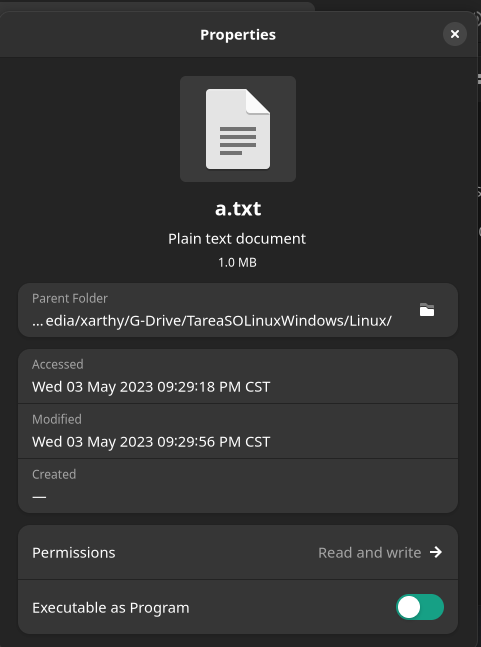
\includegraphics[scale=0.5]{/home/xarthy/operating-systems/tareaTestWindowsLinux/TareaSOLinuxWindows/Linux/Screenshot from 2023-05-03 21-31-02.png}
\end{figure}

En Windows por alguna razón el file explorer dice que pesa 977Kb, pero la terminal si dice que tiene 1000000 de bytes.

\begin{figure} [h]
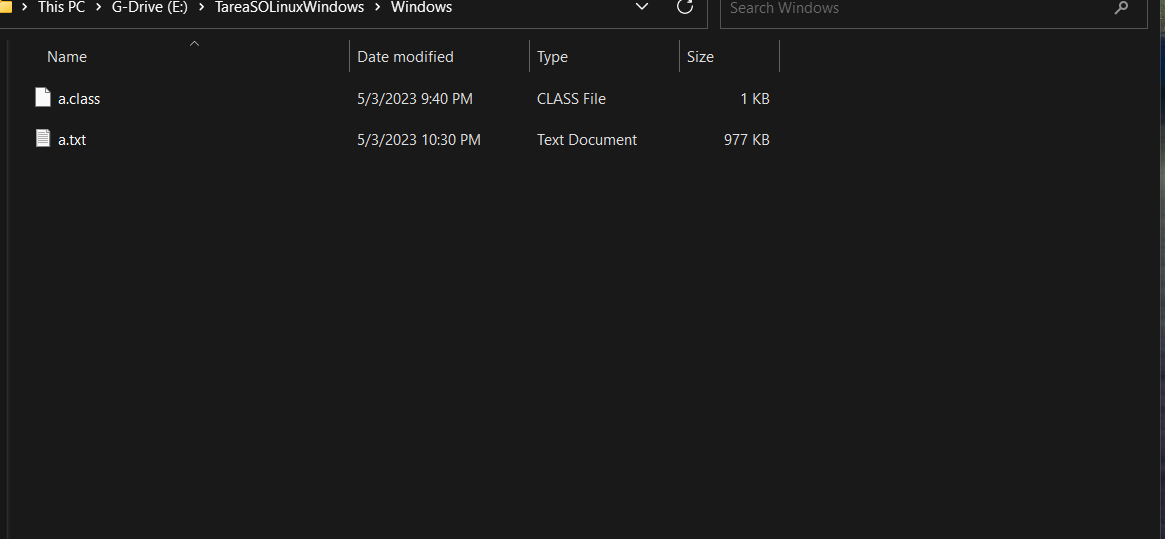
\includegraphics[width=0.5\textwidth]{/home/xarthy/operating-systems/tareaTestWindowsLinux/TareaSOLinuxWindows/Windows/Screenshot 2023-05-03 223544.png}
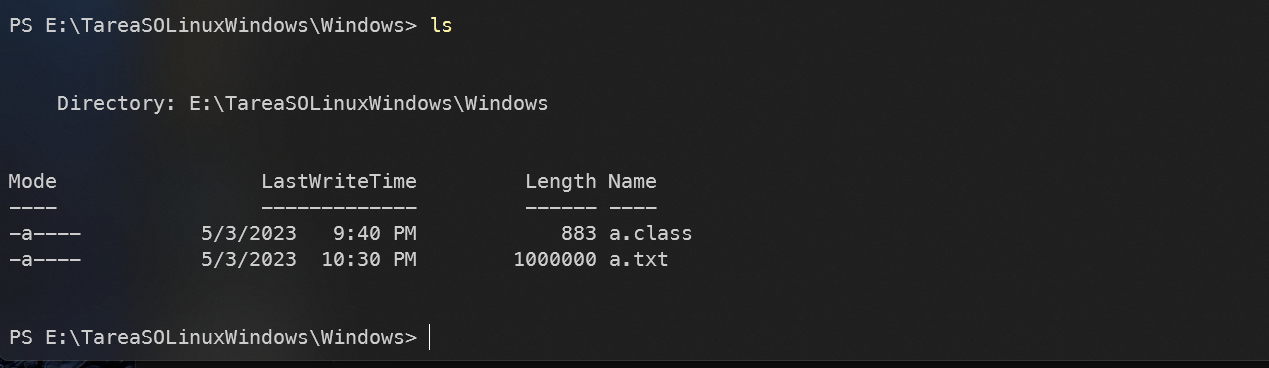
\includegraphics[width=0.5\textwidth]{/home/xarthy/operating-systems/tareaTestWindowsLinux/TareaSOLinuxWindows/Windows/Screenshot 2023-05-03 223550.png}
\end{figure}

\end{document}